\chapter{{\iqist}的安装配置}
\label{chap:install}

本章介绍如何获取、编译、安装与设置{\iqist}软件包的各个组件,在下一章将介绍如何运行{\iqist}。

\section{获取{\iqist}}
\label{sec:get}

也许您已经由中国科学院物理研究所理论室T03组的某位学生那里或者是其它途径获得了\iqist 的某个组件的源程序,
甚至还积累了不少糟糕的或者是良好的用户体验。但是需要郑重提醒您的是:{\iqist}的最新的最全的最权威的最官方
的绝对无删减版本只能通过下述途径获取。

\noindent\colorbox{pink}{\parbox[r]{\linewidth}{\quad email: huangli712@gmail.com}}

或者是

\noindent\colorbox{pink}{\parbox[r]{\linewidth}{\quad email: huangli712@yahoo.com.cn}}

出于某种考虑,我们一般不将{\iqist}对外完整发布,而只是以组件的形式独立发布{\iqist}的某个或者是某些部分。
如果您有特别的需求,请与我们联系。

请注意,如果您已经获取了{\iqist}的源代码,未经作者书面或者口头许可,建议(仅仅是建议!)您勿随意以任何方式
扩散此程序,请尊重作者的辛苦付出。用户需要遵守的协议请参阅本文的第\ref{sec:license}节。

如果您已经是{\iqist}的用户,建议您将您的名字、工作单位以及通联方式发送给我们,以便我们做用户统计。这并不
是强制性的,仅仅只是一个建议。 

\section{解压缩{\iqist}}
\label{sec:unzip}

{\iqist}的所有源文件、文档、例子都包含在名为iqist.tar.gz的压缩文件中,用一般的解压缩工具可将其解开。
以Linux系统为例,您可以用下述命令将iqist.tar.gz文件解压缩。

\noindent\colorbox{pink}{\parbox[r]{\linewidth}{\quad \$ tar xvfz iqist.tar.gz}}

如果您获取的仅仅只是{\iqist}的某个组件的源文件,例如azalea.tar.gz\footnote{{\azalea}组件的源程序。},那么
也可以用相同的命令对其进行解压:

\noindent\colorbox{pink}{\parbox[r]{\linewidth}{\quad \$ tar xvfz azalea.tar.gz}}

\section{{\iqist}的目录结构}
\label{sec:directory}

\begin{figure}
\centering
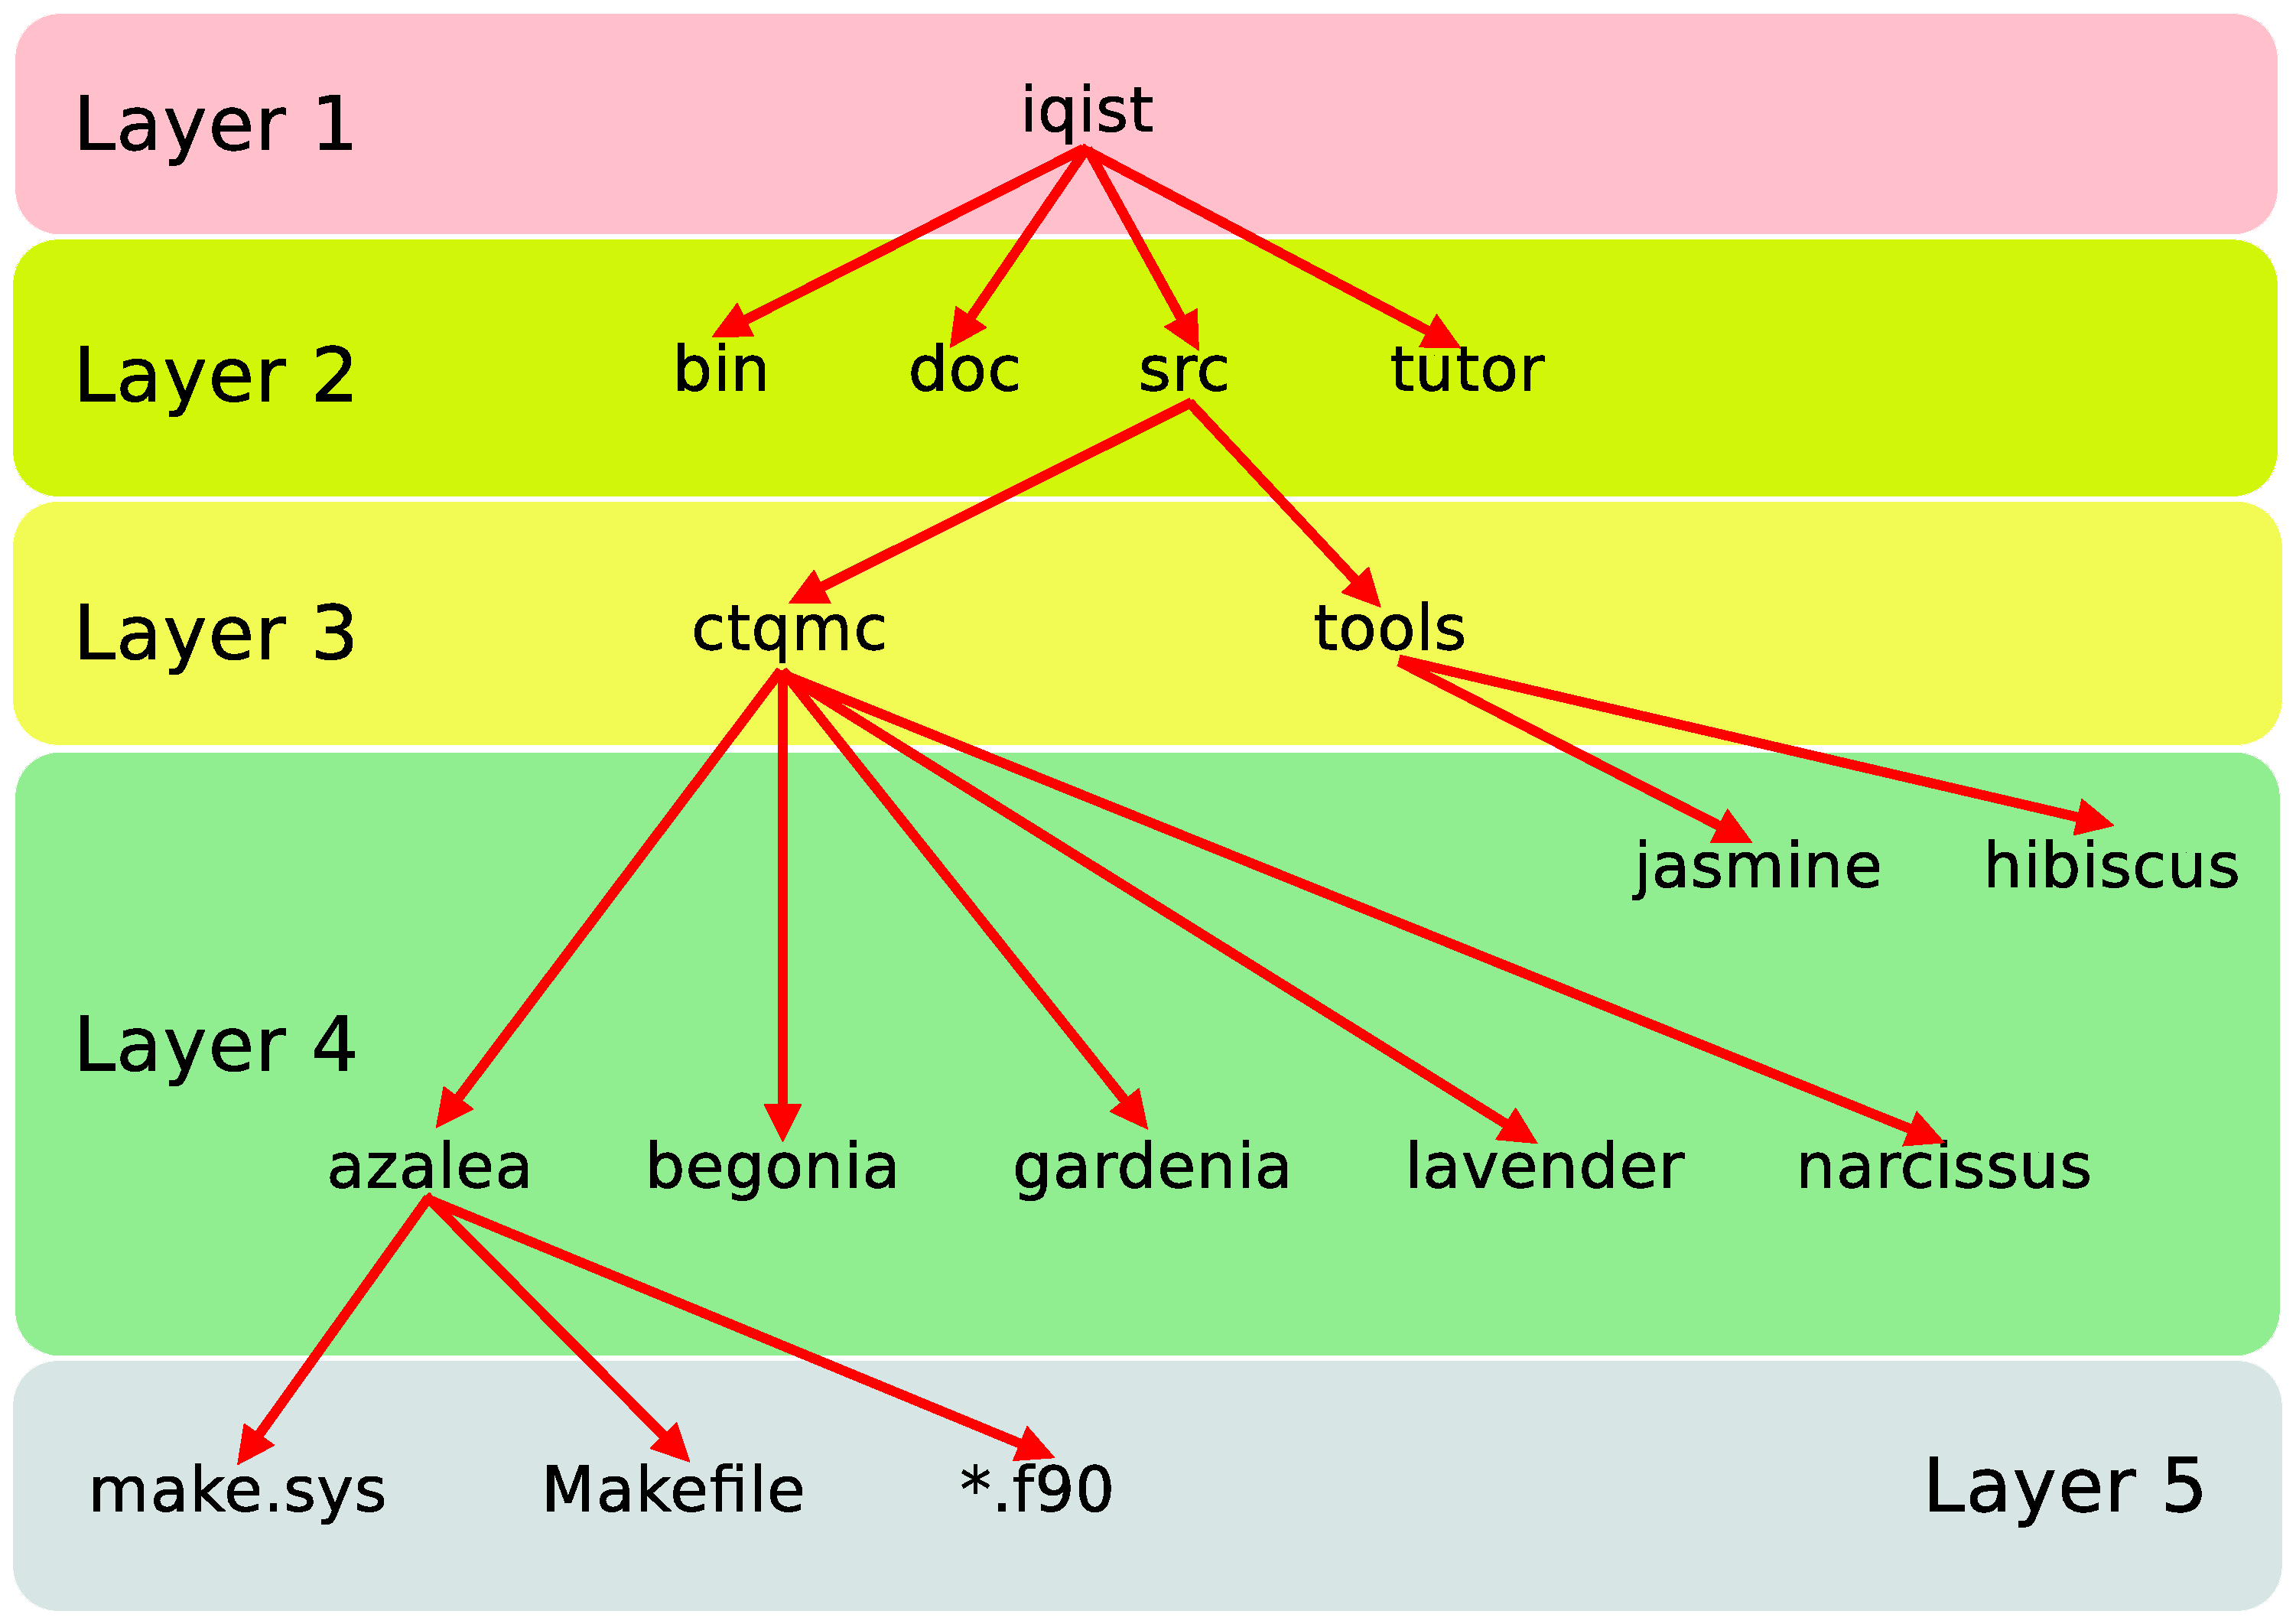
\includegraphics[scale=0.28]{figure/dir.eps}
\caption{{\iqist}软件包的目录结构\label{fig:dir}}
\end{figure}

{\iqist}的目录结构如图\ref{fig:dir}所示。每个文件夹具体存放的内容如下:
\begin{itemize}
\item bin:存放编译后可执行程序
\item doc:存放用户手册与说明文档
\item src:存放不同的组件的源程序
\item tutor:教程,提供简单的例子
\end{itemize}

在src文件夹中,又内含ctqmc与tools两个子文件夹。在ctqmc文件夹中,包含着{\azalea}、
{\gardenia}、{\narcissus}、{\begonia}与{\lavender}等组件的源程序,每个组件都有
单独的文件夹。在tools文件夹中,包含着{\jasmine}与{\hibiscus}组件的源程序,在
此目录下,还有pysci.py脚本程序。

在组件的文件夹中,有三类型文件,分别是:make.sys,Makefile,与*.f90\footnote{在{\hibiscus}组
件的目录下,还存在着以py为扩展名的Python脚本程序。}。其中*.f90为
源代码文件,不可修改。Makefile为编译主控文件,由make程序处理,不可修改。而make.sys
文件为编译设置文件,需要用户修改以适合系统的当前环境。

警告!除非您确信自己正在做些什么,并且由此可能带来的后果,否则请不要修改任
何{\iqist}组件的源代码。

\section{{\iqist}组件的编译链接}
\label{sec:compile}

{\iqist}目前并不提供一个统一的编译脚本,各个组件是分别编译链接的,也就是说,用户无法简单地敲一个命令就
把{\iqist}编译完毕。但是用户也无须感到恐惧,{\iqist}的编译链接是十分简单的。

\subsection{基本编译环境}

我们首先来看{\iqist}的编译环境。在正式编译{\iqist}之前,用户必须确保自己的系统符合以下最低要求:
\begin{itemize}
\item 操作系统为UNIX/Linux或者是Mac OS X,尽量升级为最新或者是较新的版本
\item 如果操作系统为Mac OS X,请务必提前安装Xcode套件
\item 如果操作系统为UNIX/Linux,请务必提前安装GCC套件
\item Python要求版本2.6+,安装scipy, numpy,matplotlib库\footnote{参见scipy与numpy的主
页(URL:http://www.scipy.org/)与matplotlib的主页(URL:http://matplotlib.org/)。}
\item 安装f2py\footnote{该工具负责将Python脚本与Fortran子程序耦合链接在一起(URL:http://www.scipy.org/F2py),
{\hibiscus}组件的swing程序需要用到它。}
\item 安装Intel Fortran Compiler,要求版本11.0+\footnote{关于Fortran编译器,我们推荐的是Intel提供的Fortran
编译器。从理论上说,我们的Fortran程序没有使用任何Intel Fortran独有的语法,GNU的gfortran或者PGI的pgf90应该也
是可用的,但是我们并没有对此做过测试,欢迎用户提供测试报告。将{\iqist}移植到更多的软硬件平台上是我们努力的目标之一。}
\item 安装MPI支持,MPICH1、MPICH2、OPENMPI,或者是各种定制的MPI实现均可\footnote{推荐采用ANL开发的MPICH2
的稳定版本(URL:http://www.mcs.anl.gov/research/projects/mpich2/)。}
\item 安装BLAS与LAPACK数学库\footnote{关于线性代数库有很多的选择。最简单最省事的选择是直接采用Intel提供的MKL数学
函数库。性能最差的是选择netlib上所提供的LAPACK和BLAS的标准参考实现库(URL:http://www.netlib.org/lapack/)。如果追
求性能的极致的话,BLAS的实现建议选择GotoBLAS2或者是OpenBLAS。在此隆重地向各位用户推介国人自主开发的OpenBLAS。因
为GotoBLAS2已经无人维护,它不支持最新的处理器平台以及最新的指令集。因此除非用户的机器仍旧是一些老古董,否则GotoBLAS2
已经不是一个最好的选择了。在GotoBLAS2 1.1.3BSD版本的基础上,中国科学院软件研究所并行计算实验室的张先轶等人分支出
一个新的版本,继续对其进行优化改进,并命名为OpenBLAS(URL:https://github.com/xianyi/OpenBLAS),OpenBLAS修正了不少GotoBLAS2
中的bug,新支持LLVM/clang编译器。除了最新的Intel Sandy Bridge平台外,OpenBLAS对于国产的龙芯3A/3B有着很好的支持。}
\item 安装vim、gnuplot等工具程序\footnote{参见vim的主页(URL:www.vim.org)与gnuplot的主页(URL:www.gnuplot.info)。}
\end{itemize}

\subsection{编译过程详解}

下面我们来编译{\iqist}的各个组件。此处以{\azalea}组件为例来说明编译过程,其余组件的编译过程是
完全类似的。首先进入到{\azalea}组件的源代码目录:

\noindent\colorbox{pink}{\parbox[r]{\linewidth}{\quad \$ cd iqist/src/ctqmc/azalea}}

然后使用vim编辑器编辑make.sys文件,设定编译环境:

\noindent\colorbox{pink}{\parbox[r]{\linewidth}{\quad \$ vim make.sys}}

典型的make.sys文件如下所示:

\lstset{backgroundcolor=\color{pink}, numbers=left, numberstyle=\tiny, basicstyle=\small, stringstyle=\sffamily}
\begin{lstlisting}[frame=single]
# fortran compiler and linker
#-------------------------------------------------------------------------
F90    = mpif90
LINKER = $(F90)

# fortran preprocessor options, common setting
#-------------------------------------------------------------------------
MPI    = -DMPI
OMP    = #-openmp
FPP    = -fpp
CPP    = $(FPP) $(MPI) $(OMP)

# machine tuning options, just for my laptop: iris system
#-------------------------------------------------------------------------
GPROF  = #-pg
CHECK  = -warn all #-check all -traceback -g
CDUMP  = -vec-report2 -openmp-report2 -nogen-interfaces
LEVEL  = -O3 -xHost -unroll-aggressive -align all
MTUNE  = -mtune=core2

# flags for compiler and linker
#-------------------------------------------------------------------------
FFLAGS = -c $(CPP) $(CHECK) $(CDUMP) $(LEVEL) $(MTUNE) $(GPROF)
LFLAGS = -static $(OMP) $(GPROF)

# linear algebra library, lapack and blas
#-------------------------------------------------------------------------
LIBS   = -L. -llapack -lblas #-lguide
LIBS   = -L. -llapack -lgoto #-lguide
\end{lstlisting}

我们对上面的make.sys文件稍作解释。

1.\#符号后面出现的内容表示注释,会被忽略掉。

2.第3行设定Fortran 90编译器,第4行设定链接器。

3.第8行打开MPI并行支持,如果只编译串行程序,可以注释掉该行。

4.第9行打开OpenMP并行支持,目前公布的{\iqist}组件暂不支持该技术,不要改动它。

5.第10行打开Intel Fortran Compiler内置的预处理器,这是必须的,不要改动它。
如果你的编译器不属于Intel Fortran Compiler,那么此选项可能会有所不同。

6.第15行控制是否在运行时刻采样监测运行性能,如果打开该选项将会降低性能。

7.第16行,-warn all表示在编译时刻输出所有的警告信息;-check all表示在运行时刻输出
所有监测信息,如果遇到数组越界这类型的异常会报错退出,该选项会严重降低运行效率;
-traceback选项表示在输出运行时刻出错信息时向后追朔;-g选项
表示将调试符号包含在可执行程序中,那么当程序报错时,会给出具体出错的行号。
如果你的编译器不属于Intel Fortran Compiler,那么上述选项可能会有所不同。

8.第18行,-O3、-xHost等选项都是用来设置针对当前平台产生最优化的代码。
如果你的编译器不属于Intel Fortran Compiler,那么上述选项可能会有所不同。

9.第19行设置针对core2架构产生最优的代码,如果你的处理器不属于Intel出品,或者
即使是Intel出品但是也不属于core2架构的,必须注释掉该行或者是查阅
编译器手册,将core2替换为合适的取值。我们的开发平台为core2架构,因此将其设为缺省值。
如果你的编译器不属于Intel Fortran Compiler,那么上述选项可能会有所不同。

10.第23行设置编译参数。

11.第24行设置链接参数,-static表示产生静态程序,Mac OS X系统不支持此选项。

12.第28 $\sim$ 29行,设置BLAS数学库以及LAPACK数学库的路径并将它们加入到链接选项中。选
用高度优化的BLAS与LAPACK库,例如Intel MKL、GotoBLAS2、OpenBLAS将会显著提高{\iqist}的运行
效率。注意:实际上只有第29行的设置起作用,第28行的设置被覆盖掉了。

编辑好make.sys文件后,退出vim程序。然后在命令行中用make命令编译:

\noindent\colorbox{pink}{\parbox[r]{\linewidth}{\quad \$ make}}

编译成功后,将会产生名为ctqmc的可执行程序。如果编译失败,请检查出错信息,重新编辑
make.sys文件调整编译环境。然后在命令行中输入make clean命令清除编译痕迹:

\noindent\colorbox{pink}{\parbox[r]{\linewidth}{\quad \$ make clean}}

接下来可再次用make命令进行编译。

注意:我们在上文所述的编译设置仅仅只是一个示例,仅仅只适用于开发者所使用的软硬件系统。
为了能够正确编译{\iqist},用户须根据实际情况对make.sys中的缺省设置进行微调。

\section{{\iqist}组件的安装设置}
\label{sec:setup}

按照上节中的介绍,依次编译好{\iqist}的各个组件后,用户可将可执行程序统一拷贝至iqist/bin
目录下,然后将iqist/bin目录加入到系统路径中,这样就完成了所有的安装设置工作。注意到各个
量子杂质求解器组件的可执行程序都是ctqmc,在拷贝到iqist/bin目录之前请自行重命名以防止覆盖。
